% Presentation Paper
\documentclass[11pt]{beamer}
\usepackage{color, graphics, graphicx, amsfonts, fancyhdr, makeidx, multirow}
\usepackage[english]{babel}
\usepackage[utf8]{inputenc}
\usetheme[progressbar=frametitle]{metropolis}
% \usefonttheme[onlylarge]{structurebold}
\usepackage[T1]{fontenc}
\usepackage{tabularx}
\usepackage[para,online,flushleft]{threeparttable}  
\usepackage{dcolumn} 
\usepackage{booktabs}
\usepackage{pifont}
\newcommand{\cmark}{\textcolor{green}{\ding{51}}}
\newcommand{\xmark}{\textcolor{red}{\ding{55}}}

\sloppy

\begin{document}

\title{Legislature Size and Welfare: \\ Evidence from Brazil}
\author[Mignozzetti, Cepaluni, Freire]{{Gabriel Cepaluni (UNESP), Danilo Freire (Lincoln) \& Umberto Mignozzetti (Emory)}}
\date{}

\begin{frame}
\maketitle
\end{frame}

\pagebreak

\begin{frame}{Introduction}
  \begin{itemize} \itemsep1em
   \item Institutional design 
   \item But little is known about the effect of particular legislative features on social welfare
   \item Here, we study a problem faced by all democracies, at some point in their institution building process: 
   
   \vspace{0.15in}
   
   \textbf{How many politicians should there be in their local governments?}
   
   \item But why is this problem important?
  \end{itemize}
\end{frame}

\begin{frame}{Introduction}
  \begin{itemize} \itemsep1em
   \item The number of politicians affect policy-making, taxation, checks and balances, and representation.
   \item Larger legislatures also cost a lot of money:
  \end{itemize}
  \begin{figure}[ht]
        \begin{minipage}[c]{0.45\linewidth}
            \centering
            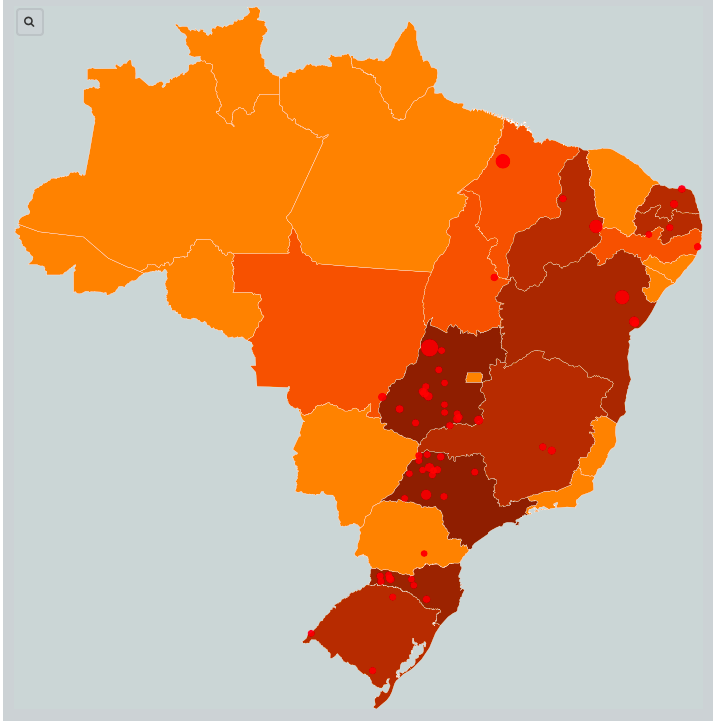
\includegraphics[width=\textwidth]{alltowns.png}
            \caption{Councils that cost more than US\$ 80.00 p.c.}
            \label{fig:a}
        \end{minipage}
        \hspace{0.5cm}
        \begin{minipage}[c]{0.45\linewidth}
            \centering
            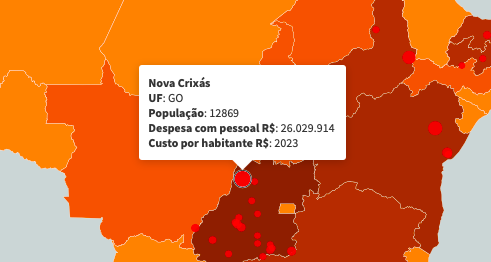
\includegraphics[width=\textwidth]{mostexpensive.png}
            \caption{Town with Highest Cost per capita: US\$ 400.00}
            \label{fig:b}
        \end{minipage}
    \end{figure}
\end{frame}

\begin{frame}
\begin{center}
\Large{\textbf{What is the effect of increasing the number of legislators on service provision?}}
\end{center}
\end{frame}

\begin{frame}{Introduction}
  \begin{itemize} \itemsep1em
   \item As there seem to be a trade-off, it is important to study in which conditions legislature size affects welfare.
   \item In this paper, we propose a model of a bargaining in a legislature to see how legislature size affects bargaining costs.
   \item We show that bargaining costs depend on the partisan composition of the legislature:
   \begin{itemize} \itemsep1em
       \item \textbf{Without partisanship}: Larger legislatures lead to higher bargaining costs.
       \item \textbf{With partisanship}: Costs depend on the policy alignment.
   \end{itemize}
  \end{itemize}
\end{frame}

\begin{frame}{Introduction}
  \begin{itemize} \itemsep1em
   \item We confirm these predictions by studying population thresholds for City Council Size in Brazil (2005-2008).
   \item We use Regression Discontinuity Design; survey data; and quantitative text analysis on 346k+ bills.
   \item We show that in the Brazilian case:
   \begin{itemize} \itemsep1em
   \item The additional city councilor belongs to the mayoral pre-electoral coalition 91\% of the time.
   \item The additional support increases the number of appointed bureaucrats, decreases infant mortality, and increases elementary school enrollment.
   \end{itemize}
  \end{itemize}
\end{frame}

\begin{frame}
\begin{center}
\Large{\textbf{Theory}}
\end{center}
\end{frame}

\begin{frame}{Number of Legislators and Welfare?}
  \begin{itemize} \itemsep1em
   \item Alchian and Demzets (1972): team productivity
   \begin{itemize}
       \item More legislators: increased productivity frontier at a moral hazard cost.
       \item The effects depend on which incentive dominates.
   \end{itemize}
   \item Weingast et al. (1981): Law of $1$/$n$
   \begin{itemize}
       \item Diffuse costs and concentrated benefits: Free-riding on common pool taxes.
       \item Overprovision (?)
   \end{itemize}
   \item Crain et al. (1979, 1982, 2012): Interest group representation.
   \begin{itemize}
       \item Mix between ease to lobby and coordination problems within legislature.
       \item Representation: more representation, better service provision.
   \end{itemize}
   \item Empirics: mixed evidences.
  \end{itemize}
\end{frame}

\begin{frame}{A Theory of Legislature Size and Welfare}
To understand the effect of legislature size, we 
propose a \textbf{legislature bargaining} game:
\begin{block}{Setup}
\begin{itemize}\itemsep1em
    \item The municipality has $R$ resources, and it is comprised of a Mayor (Executive) and a city council (Legislative).
    \item The Mayor and the City Council bargain over public goods provision and rents.
    \item And the proposal has:
    \begin{enumerate}\itemsep1em
     \item A public goods provision level ($g$)
     \item Rents for the councilors ($\textbf{x}$) and for the Mayor ($r$)
    \end{enumerate}
    \item If the simple majority of the councilors accept the proposal, it is implemented. Otherwise, it is rejected.
\end{itemize}
\end{block}
\end{frame}

\begin{frame}{A Theory of Legislature Size and Welfare}
\begin{block}{Timeline}
\begin{enumerate}  \itemsep1em
  \item The Mayor learns how many government $|G|$ and opposition $|O|$ legislators were elected.
  \item The Mayor proposes a policy vector $(r, g, \textbf{x})_M$.
  \item The City Council votes the proposal.
  \begin{itemize}
    \item If the council accepts, the policy is implemented, and the game ends. 
    \item Otherwise, the reversal policy is implemented.
  \end{itemize}
  \item (Reversal Policy) The budget is discounted by a factor $\delta \in (0,1)$, and one councilor is randomly selected to make an offer. If the offer is accepted, it is implemented. If rejected, the reversal policy stage restarts.
\end{enumerate}
\end{block}
\end{frame}

\begin{frame}{A Theory of Legislature Size and Welfare}
\begin{block}{Solution}
\begin{itemize}  \itemsep1em
  \item This game is similar to Baron and Ferejohn (1989).
  \item And we solve it for the Stationary Subgame Perfect Equilibrium.
  \item The solution consists in:
  \begin{enumerate} \itemsep1em
      \item Find a proposal that at time $k$ would make the councilor indifferent to accepting or rejecting and go to round  $k+1$.
      \item And by \textit{stationary}, we mean the proposal that would satisfy the majority of the city council at any point in time.
      \item Proceeding backwards, finding the optimal offer made by the mayor.
  \end{enumerate} \itemsep1em
  \item Here we start on step 3, for exposition purposes.
\end{itemize}
\end{block}
\end{frame}

\begin{frame}{A Theory of Legislature Size and Welfare}
\begin{block}{Governing Costs}
\begin{itemize}  \itemsep1em
  \item Councilors accept an offer that is better than wait until the next round. This generates governing costs $C_G(N)$.
  \item The Mayor knows the governing costs, and she chooses rents and public goods provision to maximize:
  \[
  \begin{aligned}
   \max_{r, g} \quad & \overbrace{u(r)}^{\substack{\text{Benefits} \\ \text{from Rents}}} + \overbrace{B_M\pi(g)}^{\substack{\text{Benefits} \\ \text{from Reelection}}}\\
   \textrm{s.t.} \quad & \underbrace{r + g + C_G(N) \leq R}_{\text{Budget constraint}}
   \end{aligned}
   \]
   \end{itemize}
  \end{block}
  \pause \begin{block}{Proposition 1}
  The provision of public goods increases with legislature size when the bargaining costs decrease with legislature size.
  \end{block}
\end{frame}

\begin{frame}{A Theory of Legislature Size and Welfare}
\begin{itemize} \itemsep1em
    \item And to determine whether the governing costs increase or decrease, we need to compute these governing costs. 
    \item It is straightforward to do that using backward induction.
    \item we solve for two mechanisms that have different underlying assumptions:
    \begin{enumerate} \itemsep1em
        \item A mechanism without partisanship, where the governing costs depend only on rents.
        \item A mechanism with partisanship, where the governing costs depend on rents and politics.
    \end{enumerate}
\end{itemize}
\end{frame}

\begin{frame}{A Theory of Legislature Size and Welfare}
\begin{block}{Baseline: Governing Costs without Partisan Concerns}
\begin{itemize} 
  \item A city councilor, in the $k$-th round of the game, accepts the proposal iff:
  \[
    \underbrace{x_i}_{\substack{\text{Current} \\ \text{offer}}} \geq \overbrace{\left(\dfrac{1}{N} \right)\left[ \delta^{k+1}R - \dfrac{N}{2}x_i \right]}^{\substack{\text{Expected} \\ \text{gains from becoming} \\ \text{the proposer}}} + \overbrace{\left( 1 - \dfrac{1}{N} \right)\left[\dfrac{1}{2} x_i \right]}^{\substack{\text{Expected} \\ \text{gains if \textbf{not}} \\ \text{the proposer}}}
 \]
 \item After some algebra, the city councilor accepts an offer in the $k$-th round iff:
 \[
  x_i \geq \dfrac{2 \delta^{k+1}R}{2N + 1}
 \]
\end{itemize}
\end{block}

\end{frame}

\begin{frame}{A Theory of Legislature Size and Welfare}
\begin{block}{Baseline: Governing Costs without Partisan Concerns}
\begin{itemize} 
  \item And at $k=0$, the Mayor has to offer at least the following amount to secure the support from a given councilor:
  \[
   x_i \geq \dfrac{2 \delta R}{2N + 1}
  \]
  \item And the governing costs are computed by offering these rents for at least half of the city councilors:
  \[
    C_G(N) \ = \ \dfrac{N}{2}\left[\dfrac{2 \delta R }{2N + 1}\right] \ = \ \dfrac{\delta R N}{2N + 1}
  \]
 \end{itemize}
 \end{block}
 \pause
 \begin{block}{Proposition 2}
   In the baseline non-partisan reversal, the bargaining costs always increase when the size of the legislature increases.
 \end{block}
\end{frame}

\begin{frame}{A Theory of Legislature Size and Welfare}
  \begin{block}{Baseline: Governing Costs without Partisan Concerns}
    \begin{figure}[htb]
      \centering
      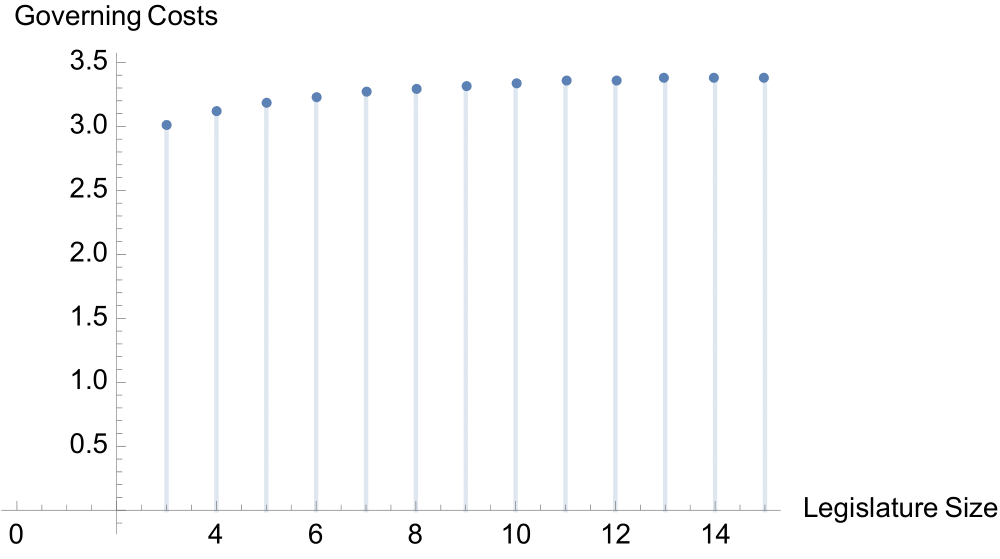
\includegraphics[width=1\textwidth]{govcostsnopart.pdf}
    \end{figure}
  \end{block}
\end{frame}

\begin{frame}{A Theory of Legislature Size and Welfare}
\begin{itemize}  \itemsep1em
  \item What happens when we add partisan concerns?
  \item There are now two types of councilors. Government councilors:
  \[
x_i + \overbrace{p}^{\substack{\text{Partisan} \\ \text{Benefit}}} \geq \dfrac{2\delta R}{2N+1}
\]
 \item And opposition councilors: 
 \[
x_i - \overbrace{p}^{\substack{\text{Partisan} \\ \text{Costs}}}  \geq \dfrac{2\delta R}{2N+1}
\]
\item And the governing costs, when the chance of electing a councilor aligned with the Mayor is $\gamma$, becomes:
\end{itemize}
\[
C_G(N) \ = \ \dfrac{N}{2}\left( \dfrac{2\delta R}{2N+1} - p \right) + \left(\dfrac{N}{2} - \gamma N \right)2p
\]
\end{frame}

\begin{frame}{A Theory of Legislature Size and Welfare}
\begin{block}{Proposition 3}
In the reversal mechanism that incorporates partisanship, if 

\[
\gamma \geq \dfrac{1}{p}\left[ \dfrac{1}{(2N+1)(2N+3)} \right] \equiv \underline{\gamma}
\]

Then the bargaining costs decrease when the legislature size increases.
\end{block}
\begin{itemize} \itemsep1em
    \item If the chances of electing a councilor aligned with the Mayor are high enough, increasing legislature size decreases the cost of governing.
    \item The corollary of this is that more legislators aligned, more public goods provision (and rents).
\end{itemize}
\end{frame}

\begin{frame}{A Theory of Legislature Size and Welfare}
  \begin{block}{Governing Costs with Partisan Concerns}
  \vspace{0.2in}
    \begin{figure}[htb]
      \centering
      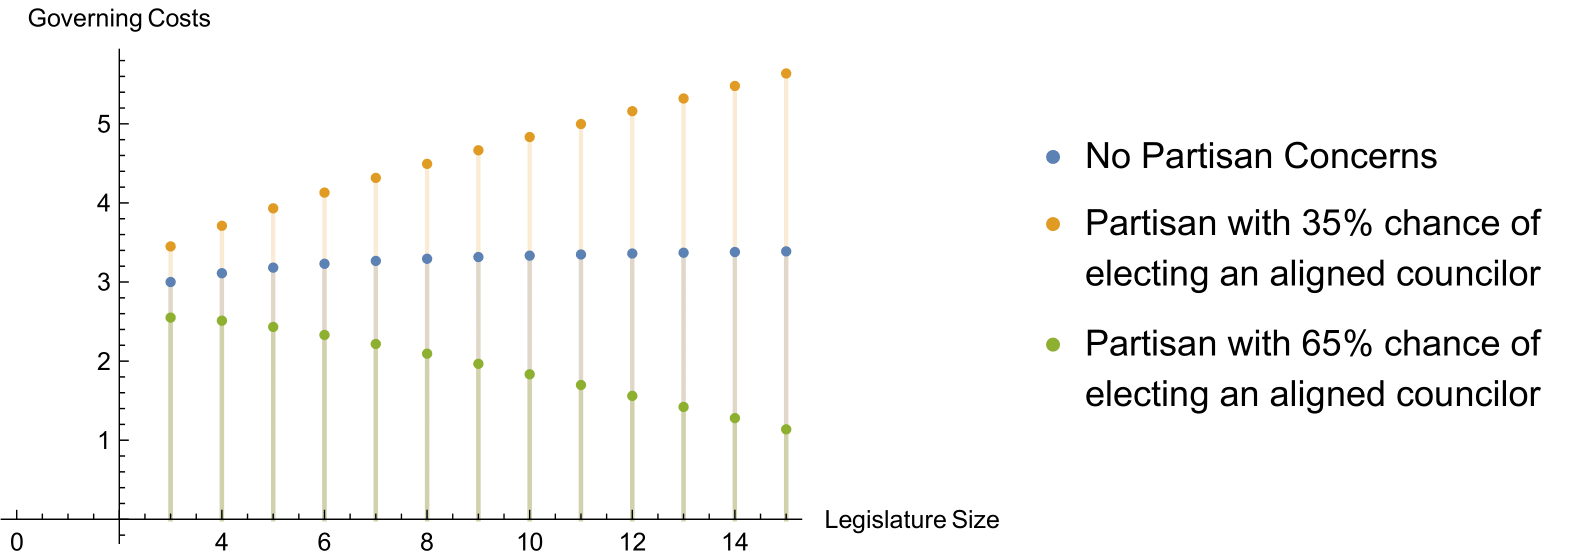
\includegraphics[width=1\textwidth]{govcostspartconcern.pdf}
    \end{figure}
  \end{block}
\end{frame}

\begin{frame}{A Theory of Legislature Size and Welfare}
To summarize:

\vspace{0.15in}

\begin{itemize} \itemsep1em
    \item Whenever the bargaining costs decrease with legislature size, public goods (and rents) increase.
    \item Without partisan concerns, bargaining costs always increase: the extra councilor needs to be paid to approve the proposal.
    \item With partisanship, the bargaining costs decrease with legislature size when the chances of electing an aligned politician are high enough.
\end{itemize}
\end{frame}


\begin{frame}
\begin{center}
\Large{\textbf{Empirics}}
\end{center}
\end{frame}

\begin{frame}{Empirical Strategy}
Brazil is the ideal test ground for this theory.
  \begin{itemize} \itemsep1em
  \item The country has wide variation in terms of welfare.
  \item The budget is mostly fixed (transfers).
  \item And city council size changed 2005 and 2008 in a way that allows me to study the effect council size on welfare.
  \item Councils before 2003:
  \end{itemize}
  \begin{table}[htp!]
\centering
\scalebox{0.8}{
\begin{tabular}{rccrrr}
  \hline\hline
 & Min. Leg. & Max. Leg. & Min. Pop. & Max. Pop. & Num. Mun. Bin \\ 
 & & & & & (2001-2004) \\
  \hline
  1 & 9  & 21 & 0 & 1,000,000 &  5,537 \\ 
  2 & 33 & 41 & 1,000,001 & 5,000,000 & 11 \\ 
  3 & 42 & 55 & 5,000,001 & $\infty$ & 2 \\ 
   \hline\hline
\end{tabular}
}
\caption{City council size thresholds 1988 Constitution}
\label{tab_city_council_size_1988}
\end{table}
\end{frame}

\begin{frame}{Empirical Strategy}
Municipalities used to define the council size inefficiently:
\begin{figure}
   \includegraphics[width=0.475\textwidth]{novasrussas.pdf}
   \hfill
   \includegraphics[width=0.475\textwidth]{sorocaba.pdf}
\end{figure}
\begin{itemize} \itemsep1em
 \item Left: Nova Russa (25,000 people e 21 councilors)
 \item Right: Sorocaba (550,000 people e 14 councilors)
\end{itemize}
\end{frame}

\begin{frame}{Empirical Strategy}
Mira Estrela (SP):
  \begin{figure}[htb]
   \centering
   \includegraphics[width=1\textwidth]{miraestrela2.pdf}
  \end{figure}
  Around 2,000 people and 11 councilors.
\end{frame}

\begin{frame}{Empirical Strategy}
Electoral Justice ruled in 2004 that:
  \begin{figure}[htb]
   \centering
   \includegraphics[width=1\textwidth]{distrSeats.pdf}
  \end{figure}
\end{frame}

\begin{frame}{Empirical Strategy}
\begin{itemize} \itemsep1em
\item Sharp RD: municipalities closer to thresholds are comparable.
\item Only difference: legislature size.
\item A perfect RDD estimation relies on three hypothesis: 
\begin{enumerate} \itemsep1em
\item Non-manipulation.
\item For multiple thresholds: the multiplicity corrections.
\item No pre-treatment variation.
\end{enumerate}
\item We developed an estimation technique for the multiple cutoffs problem.
\end{itemize}
\end{frame}

\begin{frame}{Empirical Strategy}
  \begin{figure}[htb]
   \centering
   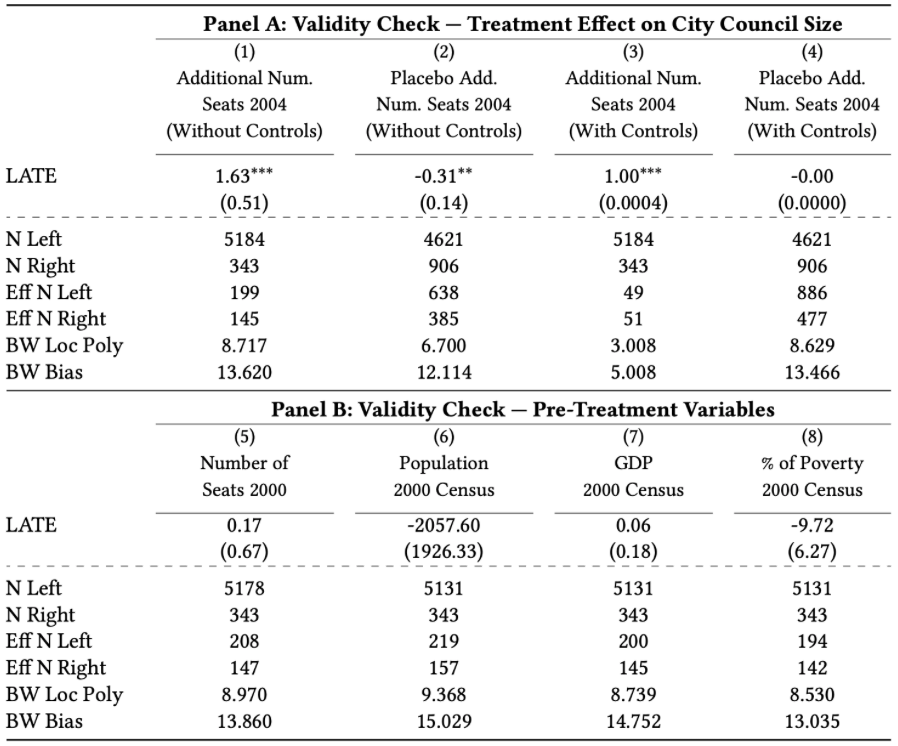
\includegraphics[width=0.9\textwidth]{fig0.png}
  \end{figure}
\end{frame}

\begin{frame}
\begin{center}
\Large{\textbf{Effect of Legislature Size on Representation and Composition of Local Chamber}}
\end{center}
\end{frame}

\begin{frame}{A Theory of Legislature Size and Welfare}
\begin{block}{Empirical Testable Hypotheses}
\begin{enumerate}
  \item[H1.] The bargaining costs decrease with legislature size when the chance of electing a government-aligned legislator is sufficiently high.
  \item[H2.] The provision of public goods increases when the bargaining costs decrease with legislature size.
\end{enumerate}
\end{block}
\pause
\begin{block}{Alternative Hypotheses}
\begin{enumerate}
  \item[AH1.] The representation of females increases with legislature size, improving public goods provision.
  \item[AH2.] The representation of non-whites increase with legislature size, improving public goods provision.
  \item[AH3.] The competitiveness of the election increases with legislature size, improving public goods provision.
  \item[AH4.] The legislative production increases with legislature size, improving public goods provision.
\end{enumerate}
\end{block}
\end{frame}

\begin{frame}{Bargaining Costs x Alternative Explanations}
  \begin{figure}[htb]
   \centering
   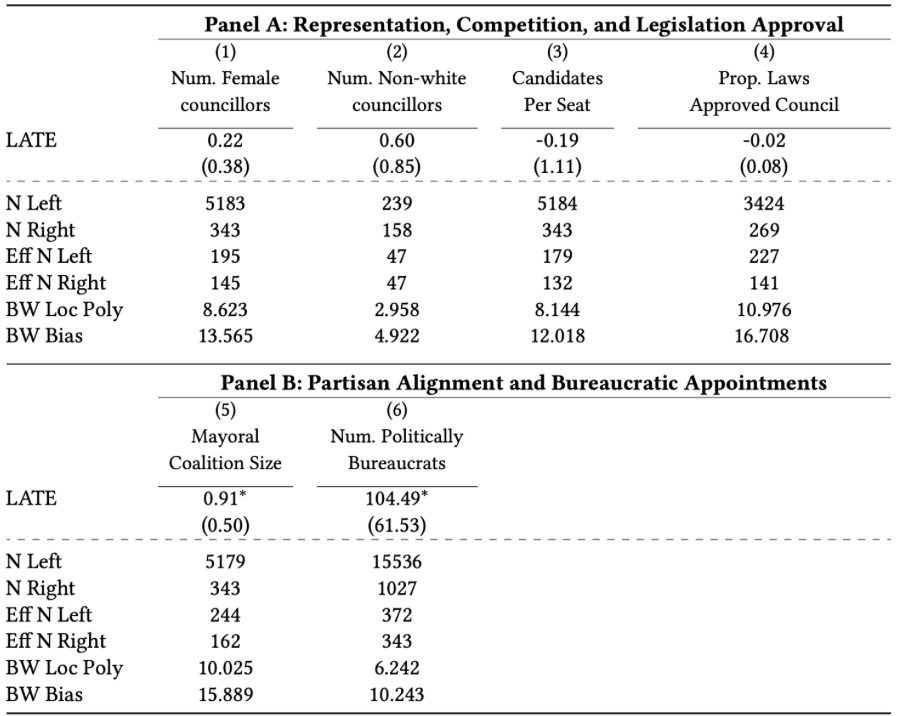
\includegraphics[width=0.9\textwidth]{fig1.png}
  \end{figure}
\end{frame}

\begin{frame}{Bargaining Costs x Alternative Explanations}
It is incentive-compatible for city councilors:
  \begin{figure}[htb]
   \centering
   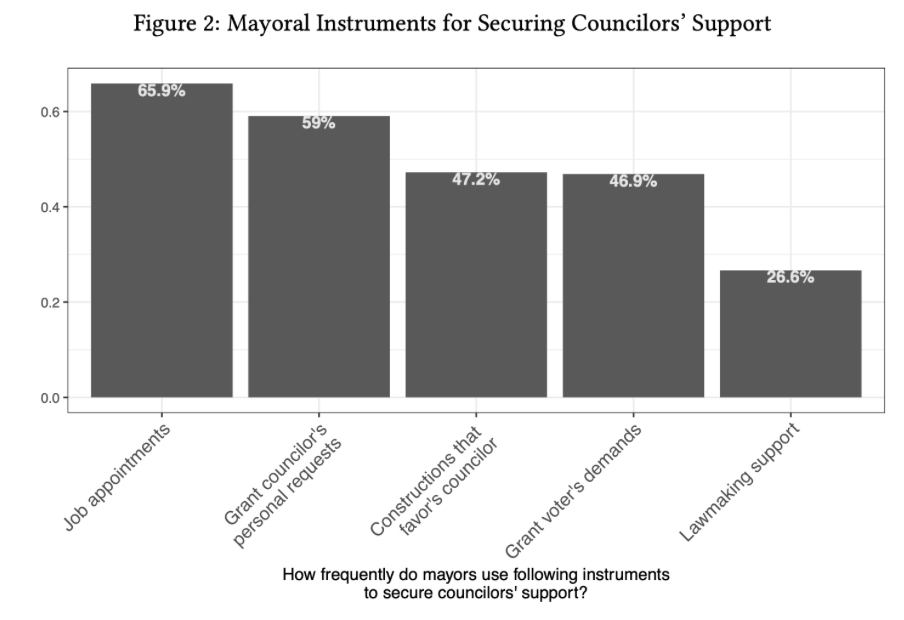
\includegraphics[width=1\textwidth]{fig2.png}
  \end{figure}
\end{frame}

\begin{frame}{Bargaining Costs x Alternative Explanations}
It reflects in the legislation approved:
  \begin{figure}[htb]
   \centering
   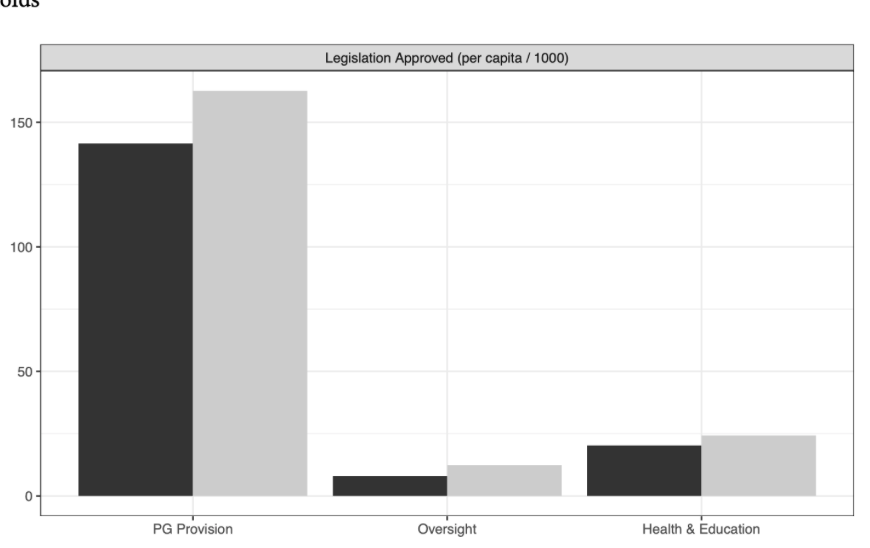
\includegraphics[width=1\textwidth]{fig3.png}
  \end{figure}
\end{frame}

\begin{frame}{Bargaining Costs x Alternative Explanations}
It reflects in the legislation approved:
  \begin{figure}[htb]
   \centering
   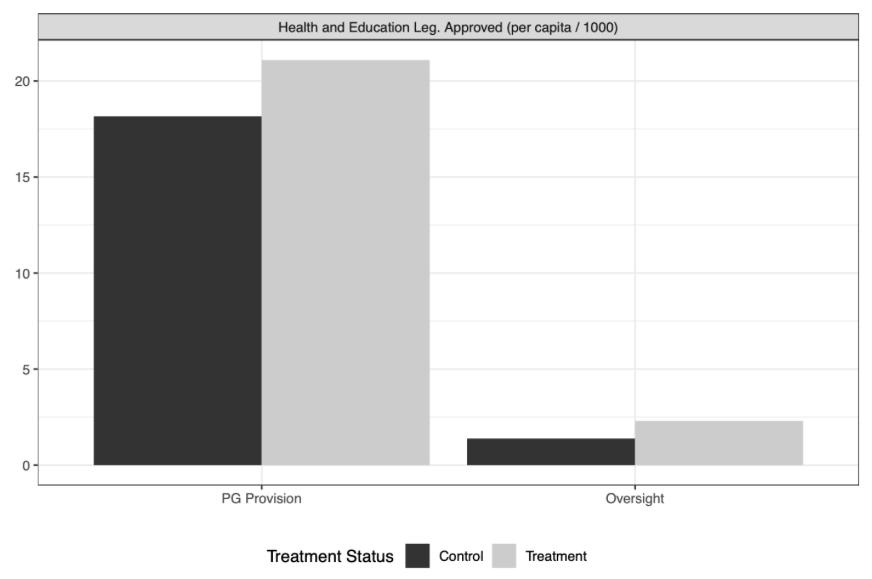
\includegraphics[width=1\textwidth]{fig4.png}
  \end{figure}
\end{frame}


\begin{frame}{Bargaining Costs x Alternative Explanations}
\begin{block}{Empirical Testable Hypotheses}
\begin{enumerate}
  \item[H1.] The bargaining costs decrease with legislature size when the chance of electing a government-aligned legislator is sufficiently high. \cmark
  \item[H2.] The provision of public goods increases when the bargaining costs decrease with legislature size.
\end{enumerate}
\end{block}
\begin{block}{Alternative Hypotheses}
\begin{enumerate}
  \item[AH1.] The representation of females increases with legislature size, improving public goods provision. \xmark
  \item[AH2.] The representation of non-whites increase with legislature size, improving public goods provision. \xmark
  \item[AH3.] The competitiveness of the election increases with legislature size, improving public goods provision. \xmark
  \item[AH4.] The legislative production increases with legislature size, improving public goods provision. \xmark
\end{enumerate}
\end{block}
\end{frame}

\begin{frame}
\begin{center}
\Large{\textbf{Effect of Legislature Size on Welfare}}
\end{center}
\end{frame}

\begin{frame}{Legislature Size and Welfare}
It also reflects on welfare:
  \begin{figure}[htb]
   \centering
   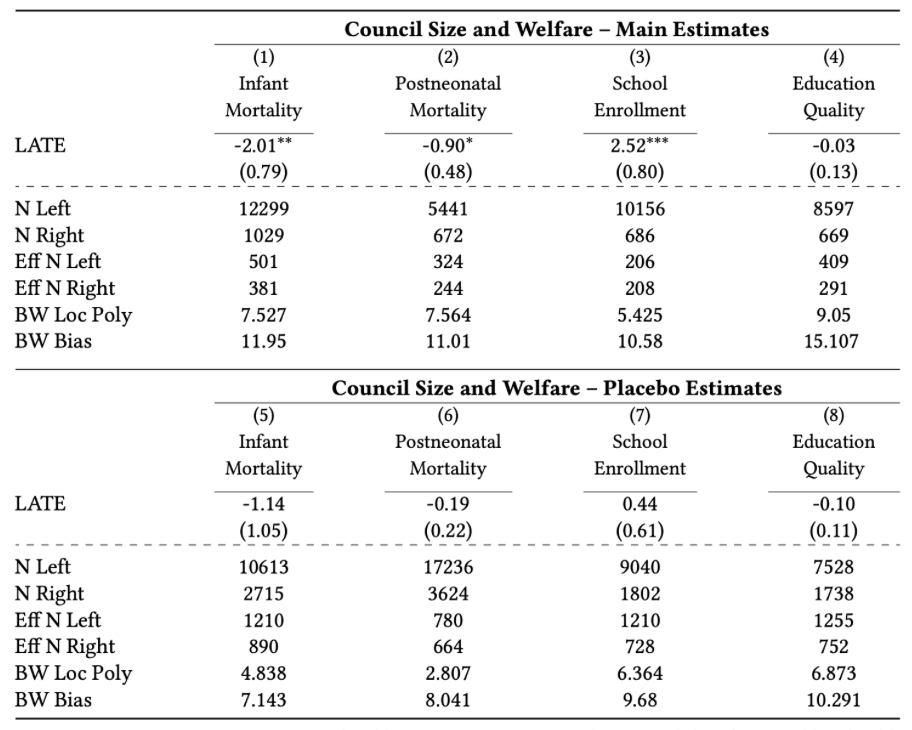
\includegraphics[width=0.8\textwidth]{fig5.png}
  \end{figure}
\end{frame}

\begin{frame}
\begin{center}
\Large{\textbf{Conclusion}}
\end{center}
\end{frame}

\begin{frame}{Conclusion}
\begin{itemize} \itemsep1em
\item When the bargaining costs decrease with legislature size, larger legislatures improve welfare.
\item In Brazil, this reflects in lower infant mortality and higher primary school enrollment. 
\item But do these results translate to other polities?
\item The best way to see the results here is through social psychology's in-group x out-group logic.

\vspace{0.15in}

\begin{enumerate} \itemsep1em
    \item Partisanship is another word for in-group x out-group tension.
    \item It is easier to reach decisions in more homogeneous groups: homogeneity decreases transaction costs.
    \item E.g.: to grab a pizza with a friend that likes pizza x with a friend that doesn't like pizza.
\end{enumerate}
\end{itemize}
\end{frame}

\begin{frame}{Conclusion}
My findings have implications for three strands in the literature:

\vspace{0.15in}

\begin{enumerate} \itemsep1em
    \item It contributes to a theory of multilateral bargaining (Baron and Ferejohn 1989; Calvert and Dietz, 2005; Choate at al. 2019; Eraslan and Evdokimov 2019).
    \item It contributes to a large literature on the effects of legislature size on public spending (Weingast et al. 1981; Primo and Snyder 2008; Alptekin et al. 2021)
    \item It also contributes to a literature on municipal party politics (Gerber and Hopkins 2011; De Benedicts-Kessner and Warshaw 2016; Frey 2020; Gouvea and Girardi 2021)
\end{enumerate}

\end{frame}

\begin{frame}
\begin{center}
\Large{\textbf{Thank you!}}
\end{center}
\end{frame}

\end{document}